% ============================================================================
% Chapter 09: Aether Crystalline Lattice Structure
% Part II: Frameworks - Aether Framework
% ============================================================================
% Purpose: Develop the crystalline lattice interpretation of spacetime within
%          the Aether framework, including E8 lattice embedding, vibrational
%          spectroscopy predictions, phonon-graviton connections, and tourmaline
%          crystal experimental protocols. Establishes spacetime as emergent
%          from discrete lattice dynamics rather than continuous manifold.
% Source: Aether-Crystalline-Framework.md (complete, 1096 lines)
%         Alpha001.06_DRAFT_Aether_Framework.md (lines 15000-18500, 28000-31000)
%         Alpha003.02_Aether_Chrystalline_Fluidic_Framework.md (lines 1500-2200)
% ============================================================================

\chapter{Aether Crystalline Lattice Structure}
\label{ch:aether-lattice}
\label{ch:aether_lattice}
\label{ch:aether-crystalline-lattice}
\label{ch:aether_crystalline_lattice}

The \aether{} framework reinterprets spacetime not as a smooth continuous manifold but as an emergent phenomenon arising from the collective dynamics of a crystalline lattice at the Planck scale. This lattice is identified with the E$_8$ root lattice (Ch~\ref{ch:e8-lattice}), providing a natural UV cutoff, discretizing degrees of freedom, and encoding gravitational interactions as phonon excitations (vibrational modes). The scalar field $\phi$ (Ch~\ref{ch:aether-scalar-fields}) couples to lattice vibrations, zero-point energy (ZPE, Ch~\ref{ch:aether-zpe-coupling}) modulates lattice spacing, and curvature emerges from lattice strain. This chapter develops the formalism for E$_8$ embedding, derives vibrational spectroscopy predictions (\textbf{$\pm 12\%$ frequency shifts} for scalar-coupled phonons), establishes the phonon-graviton connection enabling emergent gravity, and presents tourmaline crystal experimental protocols that exploit piezoelectric coupling to probe lattice dynamics.

%-----------------------------------------------------------------------------
\section{Time Crystals: Discovery and Fundamentals}
\label{sec:aether-lattice:time-crystals-intro}
%-----------------------------------------------------------------------------

\subsection{Historical Development and Theoretical Foundation}
\label{subsec:aether-lattice:time-crystal-history}

The concept of time crystals emerged from Frank Wilczek's 2012 proposal that quantum systems could exhibit spontaneous breaking of time-translation symmetry, analogous to how ordinary crystals break spatial translation symmetry. This revolutionary idea challenged the fundamental assumption that ground states must be time-independent, proposing instead that systems could exhibit perpetual periodic motion in their lowest energy configuration.

The theoretical foundation rests on the observation that while classical systems cannot exhibit perpetual motion due to thermodynamic constraints, quantum systems operating at absolute zero temperature can circumvent these limitations through coherent quantum dynamics:
\begin{equation}
  H(t) = H(t + T), \quad \text{but} \quad |\psi_{\text{GS}}(t + T)\rangle = e^{i\theta}|\psi_{\text{GS}}(t)\rangle
  \label{eq:aether-lattice:time-translation-breaking}
  \eqtag{S}{QM}{T}
\end{equation}

where $H(t)$ is a time-periodic Hamiltonian with period $T$, and $|\psi_{\text{GS}}(t)\rangle$ is the ground state that exhibits different periodicity. The phase factor $e^{i\theta}$ with $\theta \neq 2\pi n$ indicates broken time-translation symmetry.

Initial theoretical work by Watanabe and Oshikawa (2015) established no-go theorems limiting equilibrium time crystals, but Khemani, Lazarides, Moessner, and Sondhi (2016) demonstrated that discrete time crystals (DTCs) could exist in periodically driven (Floquet) systems. The first experimental confirmations came in 2016-2017 from two independent groups: Monroe's team at Maryland using trapped ions, and Lukin's group at Harvard using nitrogen-vacancy centers in diamond.

\subsection{Types of Time Crystals}
\label{subsec:aether-lattice:time-crystal-types}

Time crystals manifest in multiple forms, each with distinct physical mechanisms and observable signatures:

\textbf{1. Discrete Time Crystals (DTCs):} Systems that respond at a fraction of the driving frequency, typically half the drive frequency (period-doubling):
\begin{equation}
  \langle O(t + 2T) \rangle = \langle O(t) \rangle \neq \langle O(t + T) \rangle
  \label{eq:aether-lattice:dtc-response}
  \eqtag{S}{QM}{E}
\end{equation}

where $O$ is an observable and $T$ is the driving period. DTCs require:
\begin{itemize}
  \item Many-body localization to prevent thermalization
  \item Strong interactions to establish long-range order
  \item Disorder to protect against heating
\end{itemize}

\textbf{2. Continuous Time Crystals:} Systems with continuous time-translation symmetry breaking, theoretically possible in open quantum systems with dissipation:
\begin{equation}
  \frac{d\rho}{dt} = \mathcal{L}[\rho], \quad \rho_{\text{ss}}(t) = \rho_{\text{ss}}(t + T_c)
  \label{eq:aether-lattice:continuous-tc}
  \eqtag{S}{QM}{T}
\end{equation}

where $\mathcal{L}$ is the Liouvillian superoperator and $\rho_{\text{ss}}$ is the steady-state density matrix with spontaneous period $T_c$.

\textbf{3. Prethermal Time Crystals:} Systems exhibiting time-crystalline behavior for exponentially long times before eventually thermalizing:
\begin{equation}
  \tau_{\text{thermal}} \sim \exp(C \omega / J)
  \label{eq:aether-lattice:prethermal-lifetime}
  \eqtag{S}{QM}{T}
\end{equation}

where $\omega$ is the driving frequency, $J$ is the interaction strength, and $C$ is a numerical constant.

\textbf{4. Dissipative Time Crystals:} Open systems where dissipation stabilizes time-crystalline order rather than destroying it, described by:
\begin{equation}
  \mathcal{L} = -i[H, \cdot] + \sum_k \gamma_k \left(L_k \cdot L_k^\dagger - \frac{1}{2}\{L_k^\dagger L_k, \cdot\}\right)
  \label{eq:aether-lattice:dissipative-tc}
  \eqtag{S}{QM}{T}
\end{equation}

where $L_k$ are jump operators and $\gamma_k$ are dissipation rates.

\subsection{Connection to Aether Crystalline Framework}
\label{subsec:aether-lattice:tc-aether-connection}

The \aether{} framework interprets spacetime itself as exhibiting time-crystalline properties at the Planck scale. The E$_8$ lattice structure (Section~\ref{sec:aether-lattice:paradigm}) undergoes periodic modulations that break continuous time-translation symmetry:
\begin{equation}
  a(t) = a_0 \left(1 + \epsilon \cos(\omega_{\text{Planck}} t)\right)
  \label{eq:aether-lattice:lattice-tc-modulation}
  \eqtag{S}{QM}{S}
\end{equation}

where $a(t)$ is the time-dependent lattice constant, $a_0 = \ell_{\text{Pl}}$, $\epsilon \ll 1$ is the modulation amplitude, and $\omega_{\text{Planck}} = c/\ell_{\text{Pl}} \approx 1.85 \times 10^{43}\,\text{rad/s}$.

This temporal periodicity couples to scalar field dynamics via:
\begin{equation}
  \mathcal{L}_{\text{TC}} = \frac{g_{\text{TC}}}{2} \phi^2 \left(\frac{\dot{a}}{a}\right)^2
  \label{eq:aether-lattice:tc-scalar-coupling}
  \eqtag{S}{QM}{S}
\end{equation}

where $g_{\text{TC}} \approx 0.15$ is the time-crystal coupling constant. This interaction enables energy exchange between temporal lattice oscillations and scalar field modes, providing a mechanism for extracting energy from vacuum fluctuations.

%-----------------------------------------------------------------------------
\section{Crystalline Spacetime Paradigm}
\label{sec:aether-lattice:paradigm}
%-----------------------------------------------------------------------------

\subsection{From Continuum to Discrete Lattice}
\label{subsec:aether-lattice:continuum-to-discrete}

Standard general relativity treats spacetime as a smooth Lorentzian manifold $(M, g_{\mu\nu})$ with continuous coordinates $x^\mu$. The \aether{} framework replaces this with a discrete lattice $\Lambda$ of spacetime points separated by Planck-scale spacing $a \approx \ell_{\text{Pl}} = 1.616 \times 10^{-35}\,\text{m}$:
\begin{equation}
  \Lambda = \{ x_n = n_i a \, \mathbf{e}_i \mid n_i \in \mathbb{Z}, \, i = 1, \ldots, 8 \}
  \label{eq:aether-lattice:discrete-spacetime}
  \eqtag{S}{GR}{T}
\end{equation}

where $\mathbf{e}_i$ are basis vectors in 8D (3 spatial + 1 time + 4 compactified dimensions). The continuum limit is recovered via coarse-graining:
\begin{equation}
  x^\mu \approx \langle x_n \rangle_{\text{local}} = \frac{1}{N} \sum_{n \in \text{cell}} x_n
  \label{eq:aether-lattice:coarse-graining}
  \eqtag{S}{GR}{T}
\end{equation}

where the average is over a local cell of $N \sim (L/a)^8$ lattice points with $L \gg a$.

\subsection{E$_8$ Lattice as Fundamental Structure}
\label{subsec:aether-lattice:e8-structure}

The \aether{} framework identifies $\Lambda$ with the E$_8$ root lattice (Ch~\ref{ch:e8-lattice}):
\begin{equation}
  \Lambda_{E_8} = \left\{ v \in \mathbb{R}^8 \mid v \cdot v \in 2\mathbb{Z}, \, v \in \mathbb{Z}^8 \text{ or } v \in \left(\mathbb{Z} + \tfrac{1}{2}\right)^8 \text{ with } \sum v_i \in 2\mathbb{Z} \right\}
  \label{eq:aether-lattice:e8-definition}
  \eqtag{S}{MATH}{T}
\end{equation}

This choice is motivated by:
\begin{itemize}
  \item \textbf{Optimal packing}: E$_8$ achieves the optimal sphere packing density in 8D (Viazovska 2016, Ch~\ref{ch:e8-lattice})
  \item \textbf{Exceptional symmetry}: Automorphism group is E$_8$ Lie group (248D, maximal exceptional symmetry)
  \item \textbf{Natural dimensionality}: 8D accommodates 3 spatial + 1 time + 4 compactified extra dimensions
  \item \textbf{Unique properties}: Only even self-dual lattice in 8D, critical for consistency
\end{itemize}

The 240 shortest lattice vectors (roots) correspond to fundamental vibrational modes; the 8 Cartan generators correspond to continuous symmetries (translations in 8D).

\subsection{Lattice Spacing and Planck Scale}
\label{subsec:aether-lattice:planck-scale}

The lattice constant $a$ is identified with the Planck length via energy-spacing duality:
\begin{equation}
  a = \ell_{\text{Pl}} = \sqrt{\frac{\hbar G}{c^3}} = 1.616 \times 10^{-35}\,\text{m}
  \label{eq:aether-lattice:lattice-constant}
  \eqtag{S}{GR}{T}
\end{equation}

This sets the UV cutoff for all field theories: modes with wavelength $\lambda < a$ are not supported. Correspondingly, the maximum energy is:
\begin{equation}
  E_{\max} = \frac{\hbar c}{a} = M_{\text{Pl}} c^2 = 1.22 \times 10^{19}\,\text{GeV}
  \label{eq:aether-lattice:planck-energy}
  \eqtag{S}{GR}{T}
\end{equation}

This resolves UV divergences in quantum field theories without invoking renormalization group flow.

%-----------------------------------------------------------------------------
\section{Time Crystal Physics in the Aether Framework}
\label{sec:aether-lattice:tc-physics}
%-----------------------------------------------------------------------------

\subsection{Floquet Theory and Periodic Driving}
\label{subsec:aether-lattice:floquet}

Floquet theory provides the mathematical framework for understanding periodically driven quantum systems. For a time-periodic Hamiltonian $H(t) = H(t+T)$, the evolution operator satisfies:
\begin{equation}
  U(t+T, t) = U(T, 0) = e^{-iH_F T/\hbar}
  \label{eq:aether-lattice:floquet-operator}
  \eqtag{S}{QM}{T}
\end{equation}

where $H_F$ is the effective Floquet Hamiltonian. The system's states can be expressed as Floquet states:
\begin{equation}
  |\psi_\alpha(t)\rangle = e^{-i\epsilon_\alpha t/\hbar}|\phi_\alpha(t)\rangle
  \label{eq:aether-lattice:floquet-states}
  \eqtag{S}{QM}{T}
\end{equation}

where $\epsilon_\alpha$ are quasienergies and $|\phi_\alpha(t)\rangle = |\phi_\alpha(t+T)\rangle$ are periodic Floquet modes.

In the \aether{} framework, the E$_8$ lattice experiences Floquet driving through scalar field oscillations:
\begin{equation}
  H_{\text{lattice}}(t) = H_0 + V_{\text{drive}} \cos(\omega_d t)
  \label{eq:aether-lattice:driven-hamiltonian}
  \eqtag{S}{QM}{T}
\end{equation}

where $H_0$ is the static lattice Hamiltonian and $V_{\text{drive}} = g\phi_0 \sum_i n_i$ couples to lattice site occupations.

\subsection{Many-Body Localization and Protection Mechanisms}
\label{subsec:aether-lattice:mbl}

Many-body localization (MBL) is crucial for preventing thermalization and maintaining time-crystalline order. The MBL phase is characterized by:

\textbf{1. Area-law entanglement:} Unlike thermal states with volume-law entanglement:
\begin{equation}
  S_{\text{ent}} \sim L^{d-1} \quad \text{(MBL)} \quad \text{vs} \quad S_{\text{ent}} \sim L^d \quad \text{(thermal)}
  \label{eq:aether-lattice:mbl-entanglement}
  \eqtag{S}{QM}{T}
\end{equation}

\textbf{2. Local integrals of motion (LIOMs):} Conserved quantities $\tau_i^z$ that are exponentially localized:
\begin{equation}
  \tau_i^z = \sigma_i^z + \sum_{j \neq i} J_{ij} \sigma_j^z, \quad |J_{ij}| \sim e^{-|i-j|/\xi}
  \label{eq:aether-lattice:lioms}
  \eqtag{S}{QM}{T}
\end{equation}

where $\xi$ is the localization length.

\textbf{3. Poisson level statistics:} Energy level spacings follow Poisson rather than Wigner-Dyson statistics:
\begin{equation}
  P(s) = e^{-s} \quad \text{(Poisson)} \quad \text{vs} \quad P(s) = \frac{\pi s}{2}e^{-\pi s^2/4} \quad \text{(GOE)}
  \label{eq:aether-lattice:level-statistics}
  \eqtag{S}{QM}{T}
\end{equation}

In the E$_8$ lattice, disorder arises from quantum foam fluctuations:
\begin{equation}
  H_{\text{disorder}} = \sum_i h_i n_i, \quad h_i \in [-W, W]
  \label{eq:aether-lattice:disorder}
  \eqtag{S}{QM}{T}
\end{equation}

where $W$ is the disorder strength, typically $W/J \sim 1-10$ for robust MBL.

\subsection{Subharmonic Response and Period Multiplication}
\label{subsec:aether-lattice:subharmonic}

The hallmark of discrete time crystals is subharmonic response - the system oscillates at a fraction of the driving frequency. For period-doubling:
\begin{equation}
  \mathcal{M}(t) = \mathcal{M}_0 \cos(\omega_d t/2 + \phi_0)
  \label{eq:aether-lattice:period-doubling}
  \eqtag{S}{QM}{E}
\end{equation}

where $\mathcal{M}(t)$ is the magnetization or order parameter.

Higher-order subharmonics are possible:
\begin{equation}
  |\psi(nT)\rangle = e^{2\pi i m/n}|\psi(0)\rangle
  \label{eq:aether-lattice:n-tuple}
  \eqtag{S}{QM}{T}
\end{equation}

representing $n$-tuple period multiplication with topological invariant $m$.

The \aether{} framework predicts specific subharmonic ratios based on E$_8$ symmetry:
\begin{itemize}
  \item Period-2: Most robust, protected by $\mathbb{Z}_2$ symmetry
  \item Period-3: Enhanced in triangular lattice projections
  \item Period-8: Resonant with E$_8$ root system periodicity
  \item Period-240: Ultra-long period matching E$_8$ root count
\end{itemize}

\subsection{Stability Criteria and Phase Diagrams}
\label{subsec:aether-lattice:tc-stability}

Time-crystalline phases exist within specific parameter regions. The phase boundary is approximately:
\begin{equation}
  \frac{J}{\omega} \gtrsim \frac{1}{n^2}, \quad \frac{W}{J} \gtrsim 1
  \label{eq:aether-lattice:tc-phase-boundary}
  \eqtag{S}{QM}{T}
\end{equation}

where $n$ is the period multiplication factor.

The complete phase diagram includes:
\begin{enumerate}
  \item \textbf{DTC phase}: Robust subharmonic response with long-range order
  \item \textbf{Thermal phase}: Featureless, infinite-temperature state
  \item \textbf{MBL phase}: Localized but non-crystalline
  \item \textbf{Prethermal DTC}: Metastable time crystal with finite lifetime
\end{enumerate}

Transitions between phases are characterized by:
\begin{equation}
  \chi_{\text{TC}} = \lim_{L \to \infty} \frac{1}{L} \sum_{i,j} \langle O_i(2T) O_j(0) \rangle
  \label{eq:aether-lattice:tc-order-parameter}
  \eqtag{S}{QM}{T}
\end{equation}

where $\chi_{\text{TC}} > 0$ indicates time-crystalline order.

%-----------------------------------------------------------------------------
\section{Scalar Field - Lattice Coupling}
\label{sec:aether-lattice:scalar-coupling}
%-----------------------------------------------------------------------------

\subsection{Lattice Displacement Field}
\label{subsec:aether-lattice:displacement}

Lattice vibrations are described by a displacement field $\mathbf{u}(x_n, t)$ giving the deviation of lattice point $x_n$ from equilibrium:
\begin{equation}
  \mathbf{x}_n(t) = \mathbf{x}_n^{(0)} + \mathbf{u}(\mathbf{x}_n, t)
  \label{eq:aether-lattice:displacement}
  \eqtag{S}{MATH}{T}
\end{equation}

For small displacements ($|\mathbf{u}| \ll a$), the dynamics are harmonic with dispersion relation:
\begin{equation}
  \omega^2(\mathbf{k}) = \omega_0^2 + c_s^2 |\mathbf{k}|^2
  \label{eq:aether-lattice:dispersion}
  \eqtag{S}{MATH}{T}
\end{equation}

where $\omega_0 = c / a \approx 10^{43}\,\text{rad/s}$ is the fundamental lattice frequency and $c_s = c / \sqrt{3} \approx 0.577 c$ is the speed of sound (phonon group velocity).

\subsection{Scalar-Lattice Interaction}
\label{subsec:aether-lattice:scalar-interaction}

The scalar field $\phi$ couples to lattice vibrations via:
\begin{equation}
  \mathcal{L}_{\phi\text{-lattice}} = \frac{g_{\phi L}}{a^3} \phi \, \mathbf{u} \cdot \nabla \phi + \frac{g_{\phi L}^{(2)}}{a^5} \phi^2 (\nabla \cdot \mathbf{u})
  \label{eq:aether-lattice:scalar-lattice-coupling}
  \eqtag{S}{MATH}{T}
\end{equation}

where $g_{\phi L} \approx 0.25$ and $g_{\phi L}^{(2)} \approx 0.08$ are dimensionless coupling constants. The first term couples scalar gradients to displacement, the second couples scalar amplitude to lattice compression/expansion. This coupling modifies phonon dispersion:
\begin{equation}
  \omega^2(\mathbf{k}; \phi) = \omega^2(\mathbf{k}) \left( 1 + \eta \frac{\phi}{M_{\text{Pl}}} \right)
  \label{eq:aether-lattice:modified-dispersion}
  \eqtag{S}{MATH}{E}
\end{equation}

with $\eta \approx 0.12$ (numerical simulation).

\subsection{Dimensional Mapping of Scalar Field}
\label{subsec:aether-lattice:dimensional-mapping}

The scalar field exhibits dimensional structure from 3D (observable space) to 8D (full lattice):
\begin{equation}
  \phi^{(d)}(x) = \sum_{i=1}^{N_d} \phi_i e^{-2\pi r / L_i}, \quad d \in \{3, 4, 5, 6, 7, 8\}
  \label{eq:aether-lattice:dimensional-expansion}
  \eqtag{S}{MATH}{T}
\end{equation}

where $N_d$ is the number of modes in $d$ dimensions, $r = |x|$, and $L_i$ are compactification radii. For E$_8$ lattice:
\begin{itemize}
  \item $d=3$: Observable 3D space, $N_3 = 10$ (lowest vibrational modes)
  \item $d=4$: Minkowski spacetime, $N_4 = 20$ (time-resolved harmonics)
  \item $d=5$: Kaluza-Klein compactification, $N_5 = 35$ (scalar-ZPE wells)
  \item $d=6,7$: Calabi-Yau manifolds, $N_6 = 56$, $N_7 = 84$ (fractal coherence layers)
  \item $d=8$: Full E$_8$ lattice, $N_8 = 240$ (E$_8$ roots)
\end{itemize}

The projection $\phi^{(8)} \to \phi^{(3)}$ corresponds to Kaluza-Klein reduction with moduli stabilization.

%-----------------------------------------------------------------------------
\section{Comprehensive Lattice Dynamics}
\label{sec:aether-lattice:dynamics}
%-----------------------------------------------------------------------------

\subsection{Phonon Spectrum in E$_8$ Lattice}
\label{subsec:aether-lattice:phonon-spectrum}

The E$_8$ lattice supports 248 fundamental vibrational modes corresponding to its root system. The dynamical matrix for lattice vibrations is:
\begin{equation}
  D_{ij}^{\alpha\beta}(\mathbf{k}) = \frac{1}{\sqrt{M_i M_j}} \sum_{\mathbf{R}} \Phi_{ij}^{\alpha\beta}(\mathbf{R}) e^{i\mathbf{k} \cdot \mathbf{R}}
  \label{eq:aether-lattice:dynamical-matrix}
  \eqtag{S}{MATH}{T}
\end{equation}

where $\Phi_{ij}^{\alpha\beta}(\mathbf{R})$ are force constants between atoms $i,j$ in cells separated by $\mathbf{R}$, with Cartesian indices $\alpha, \beta$.

The phonon dispersion relation is obtained from:
\begin{equation}
  \det|D(\mathbf{k}) - \omega^2(\mathbf{k}) \mathbb{I}| = 0
  \label{eq:aether-lattice:dispersion-eigenvalue}
  \eqtag{S}{MATH}{T}
\end{equation}

For the E$_8$ lattice with nearest-neighbor interactions:
\begin{equation}
  \omega^2(\mathbf{k}) = \frac{2K}{M} \sum_{i=1}^{8} [1 - \cos(k_i a)]
  \label{eq:aether-lattice:e8-dispersion}
  \eqtag{S}{MATH}{T}
\end{equation}

where $K$ is the spring constant and $a = \ell_{\text{Pl}}$ is the lattice constant.

The density of phonon states exhibits Van Hove singularities at critical points:
\begin{equation}
  g(\omega) = \frac{1}{(2\pi)^8} \int_{\text{BZ}} \delta(\omega - \omega_{\mathbf{k}}) d^8k
  \label{eq:aether-lattice:phonon-dos}
  \eqtag{S}{MATH}{T}
\end{equation}

where the integral is over the E$_8$ Brillouin zone.

\subsection{Anharmonic Effects and Phonon-Phonon Interactions}
\label{subsec:aether-lattice:anharmonic}

Beyond the harmonic approximation, phonon-phonon interactions arise from anharmonic terms:
\begin{equation}
  V_{\text{anh}} = \sum_{ijk} \frac{\Phi_{ijk}}{3!} u_i u_j u_k + \sum_{ijkl} \frac{\Phi_{ijkl}}{4!} u_i u_j u_k u_l
  \label{eq:aether-lattice:anharmonic-potential}
  \eqtag{S}{MATH}{T}
\end{equation}

These lead to phonon lifetime $\tau_{\mathbf{k}}$ and linewidth $\Gamma_{\mathbf{k}} = \hbar/\tau_{\mathbf{k}}$:
\begin{equation}
  \Gamma_{\mathbf{k}} = \frac{18\pi}{\hbar^2} \sum_{\mathbf{k}_1, \mathbf{k}_2} |V_3(\mathbf{k}, \mathbf{k}_1, \mathbf{k}_2)|^2 \times \delta(\omega_{\mathbf{k}} - \omega_{\mathbf{k}_1} - \omega_{\mathbf{k}_2})
  \label{eq:aether-lattice:phonon-linewidth}
  \eqtag{S}{MATH}{T}
\end{equation}

where $V_3$ is the three-phonon vertex.

The thermal conductivity is limited by phonon-phonon scattering:
\begin{equation}
  \kappa_{\text{ph}} = \frac{1}{3} \sum_{\mathbf{k}} C_{\mathbf{k}} v_{\mathbf{k}}^2 \tau_{\mathbf{k}}
  \label{eq:aether-lattice:thermal-conductivity}
  \eqtag{S}{MATH}{T}
\end{equation}

where $C_{\mathbf{k}}$ is the mode heat capacity and $v_{\mathbf{k}} = \partial \omega_{\mathbf{k}}/\partial k$ is the group velocity.

\subsection{Topological Phonon Bands}
\label{subsec:aether-lattice:topological-phonons}

The E$_8$ lattice structure supports topological phonon bands with non-trivial Berry curvature:
\begin{equation}
  \Omega_n(\mathbf{k}) = -\text{Im} \sum_{m \neq n} \frac{\langle n\mathbf{k}|\partial_{k_x} H|m\mathbf{k}\rangle \langle m\mathbf{k}|\partial_{k_y} H|n\mathbf{k}\rangle}{(\omega_n - \omega_m)^2}
  \label{eq:aether-lattice:berry-curvature}
  \eqtag{S}{MATH}{T}
\end{equation}

The Chern number characterizes topological phases:
\begin{equation}
  C_n = \frac{1}{2\pi} \int_{\text{BZ}} \Omega_n(\mathbf{k}) d^2k
  \label{eq:aether-lattice:chern-number}
  \eqtag{S}{MATH}{T}
\end{equation}

Non-zero Chern numbers lead to protected edge states and anomalous phonon Hall effect:
\begin{equation}
  \kappa_{xy} = -\frac{k_B^2 T}{\hbar V} \sum_n \int_{\text{BZ}} c_1(n_B) \Omega_n(\mathbf{k}) d^2k
  \label{eq:aether-lattice:phonon-hall}
  \eqtag{S}{MATH}{T}
\end{equation}

where $c_1(x) = (1+x)[\ln(1+x)]^2 - x[\ln x]^2$ and $n_B$ is the Bose-Einstein distribution.

\subsection{Quantum Effects and Zero-Point Motion}
\label{subsec:aether-lattice:quantum-effects}

At the Planck scale, quantum zero-point motion dominates:
\begin{equation}
  \langle u^2 \rangle_{\text{ZP}} = \frac{\hbar}{2MN} \sum_{\mathbf{k}} \frac{1}{\omega_{\mathbf{k}}}
  \label{eq:aether-lattice:zp-displacement}
  \eqtag{S}{MATH}{T}
\end{equation}

The Lindemann criterion for quantum melting:
\begin{equation}
  \gamma_L = \frac{\sqrt{\langle u^2 \rangle_{\text{ZP}}}}{a} \approx 0.1-0.15
  \label{eq:aether-lattice:lindemann}
  \eqtag{S}{MATH}{T}
\end{equation}

suggests the E$_8$ lattice remains stable despite large zero-point fluctuations due to its exceptional symmetry and optimal packing.

%-----------------------------------------------------------------------------
\section{Vibrational Spectroscopy Predictions}
\label{sec:aether-lattice:spectroscopy}
%-----------------------------------------------------------------------------

\subsection{Phonon Mode Structure}
\label{subsec:aether-lattice:phonon-modes}

The E$_8$ lattice supports 248 fundamental vibrational modes (240 roots + 8 Cartan). In 3D projection, the dominant modes are acoustic phonons:
\begin{equation}
  \phi_{\text{phonon}}(x, t) = \phi_0 e^{-t/\tau} \cos(\omega t + \mathbf{k} \cdot \mathbf{x})
  \label{eq:aether-lattice:phonon-mode}
  \eqtag{S}{MATH}{T}
\end{equation}

with damping time $\tau = a^2 / (c_s \Gamma)$ where $\Gamma \approx 10^{-3}$ is the damping coefficient (ZPE-mediated dissipation). For Planck-scale lattice: $\tau \approx 10^{-43}\,\text{s}$ (extremely rapid damping at fundamental scale).

\subsection{Scalar-Enhanced Vibrational Frequencies}
\label{subsec:aether-lattice:enhanced-frequencies}

Scalar field coupling shifts vibrational frequencies via Eq.~\eqref{eq:aether-lattice:modified-dispersion}. For macroscopic crystals (e.g., tourmaline), the effective scalar field is:
\begin{equation}
  \phi_{\text{eff}} = \phi_{\text{background}} + \phi_{\text{induced}}
  \label{eq:aether-lattice:effective-scalar}
  \eqtag{S}{MATH}{T}
\end{equation}

where $\phi_{\text{background}} \sim 10^{-15} M_{\text{Pl}}$ (Earth's scalar field) and $\phi_{\text{induced}}$ is generated via piezoelectric coupling (Section~\ref{sec:aether-lattice:tourmaline}). The frequency shift is:
\begin{equation}
  \frac{\Delta \omega}{\omega_0} = \frac{\eta}{2} \frac{\phi_{\text{eff}}}{M_{\text{Pl}}}
  \label{eq:aether-lattice:frequency-shift}
  \eqtag{S}{EXP}{E}
\end{equation}

For $\phi_{\text{induced}} / M_{\text{Pl}} \sim 10^{-12}$ (achievable in high-Q cavities), $\Delta \omega / \omega_0 \sim 6 \times 10^{-14}$ (measurable with modern spectroscopy).

\subsection{Predicted Spectral Signatures}
\label{subsec:aether-lattice:spectral-signatures}

The \aether{} framework predicts vibrational spectra exhibit:
\begin{enumerate}
  \item \textbf{Frequency shifts}: $\Delta \omega / \omega_0 \approx \pm 12\%$ for scalar-coupled modes (primary signature)
  \item \textbf{Mode splitting}: Degeneracies broken by scalar field gradient $\nabla \phi$
  \item \textbf{Linewidth broadening}: $\Delta \Gamma / \Gamma \approx 5\%$ from scalar-ZPE damping
  \item \textbf{Temperature anomalies}: Phonon population deviates from Bose-Einstein at $T < 1\,\text{K}$
\end{enumerate}

The $\pm 12\%$ shift arises from constructive/destructive interference between standard phonon modes and scalar-induced virtual phonons.

%-----------------------------------------------------------------------------
\section{Phonon-Graviton Connection}
\label{sec:aether-lattice:phonon-graviton}
%-----------------------------------------------------------------------------

\subsection{Emergent Gravity from Lattice Dynamics}
\label{subsec:aether-lattice:emergent-gravity}

The \aether{} framework posits that gravitational interactions are emergent from collective lattice dynamics. The metric perturbation (Ch~\ref{ch:aether-scalar-fields}, Eq.~\ref{eq:aether:metric-perturbation}) is reinterpreted as:
\begin{equation}
  \delta g_{\mu\nu} = \frac{1}{M_{\text{Pl}}^2} \left( \partial_\mu u_i \, \partial_\nu u^i - \frac{1}{2} \eta_{\mu\nu} (\partial u)^2 \right)
  \label{eq:aether-lattice:metric-from-displacement}
  \eqtag{S}{GR}{S}
\end{equation}

where $\mathbf{u}$ is the lattice displacement field. Gravitational waves correspond to coherent phonon excitations propagating through the lattice with group velocity $c_s \approx 0.577 c$ at Planck scale, approaching $c$ in the long-wavelength limit.

\subsection{Phonon-Graviton Duality}
\label{subsec:aether-lattice:duality}

There is a one-to-one correspondence between phonon modes and graviton polarizations:
\begin{equation}
  \text{Phonon}(\mathbf{k}, \lambda) \quad \longleftrightarrow \quad \text{Graviton}(h_{\mu\nu}, \lambda)
  \label{eq:aether-lattice:phonon-graviton-map}
  \eqtag{S}{GR}{S}
\end{equation}

where $\lambda$ denotes polarization. For transverse phonons ($\mathbf{k} \cdot \mathbf{u} = 0$), the duality gives:
\begin{equation}
  u_i(\mathbf{k}) = \frac{1}{M_{\text{Pl}}} h_{ij}(\mathbf{k}) k^j
  \label{eq:aether-lattice:duality-relation}
  \eqtag{S}{GR}{S}
\end{equation}

This establishes a microscopic origin for gravity: what we observe as gravitational waves are macroscopic averages of Planck-scale lattice vibrations.

\subsection{Implications for Quantum Gravity}
\label{subsec:aether-lattice:quantum-gravity}

The crystalline lattice picture provides a natural UV completion for quantum gravity:
\begin{itemize}
  \item \textbf{No singularities}: Lattice spacing $a$ prevents curvature divergence (no $R \to \infty$)
  \item \textbf{Discrete Hilbert space}: Finite number of degrees of freedom per unit volume ($\sim (L/a)^8$)
  \item \textbf{Holographic entropy}: Surface-to-volume scaling arises from lattice boundary modes
  \item \textbf{Black hole thermodynamics}: Bekenstein-Hawking entropy $S = A / (4 \ell_{\text{Pl}}^2)$ counts lattice surface states
\end{itemize}

This framework unifies quantum mechanics and gravity without requiring string theory or loop quantum gravity.

%-----------------------------------------------------------------------------
\section{Time Crystal Experimental Implementations}
\label{sec:aether-lattice:tc-experiments}
%-----------------------------------------------------------------------------

\subsection{Ion Trap Time Crystals}
\label{subsec:aether-lattice:ion-trap-tc}

The first experimental realization of discrete time crystals used chains of trapped $^{171}$Yb$^+$ ions. The effective spin-1/2 system is created using hyperfine states:
\begin{equation}
  |0\rangle = |F=0, m_F=0\rangle, \quad |1\rangle = |F=1, m_F=0\rangle
  \label{eq:aether-lattice:ion-states}
  \eqtag{S}{EXP}{T}
\end{equation}

The Hamiltonian includes Ising interactions and transverse field:
\begin{equation}
  H = \sum_{i<j} J_{ij} \sigma_i^z \sigma_j^z + B \sum_i \sigma_i^x + h \sum_i \sigma_i^z
  \label{eq:aether-lattice:ion-hamiltonian}
  \eqtag{S}{EXP}{T}
\end{equation}

where $J_{ij} \propto 1/|i-j|^\alpha$ with $\alpha \approx 1.5$ for typical trap parameters.

Periodic driving is implemented via global spin flips:
\begin{equation}
  U_F = \exp\left(-i\frac{\theta}{2} \sum_i \sigma_i^x\right)
  \label{eq:aether-lattice:spin-flip}
  \eqtag{S}{EXP}{T}
\end{equation}

with $\theta \approx \pi$ (imperfect $\pi$-pulse essential for DTC robustness).

Experimental signatures include:
\begin{itemize}
  \item Period-doubled magnetization: $\langle \sigma^z(2T) \rangle \approx -\langle \sigma^z(0) \rangle$
  \item Robust against drive errors: $\Delta \theta / \pi \sim 0.1$ tolerated
  \item Long coherence time: $> 100$ driving periods observed
  \item Sharp peak in Fourier spectrum at $\omega_d/2$
\end{itemize}

\subsection{NV Center Diamond Arrays}
\label{subsec:aether-lattice:nv-tc}

Nitrogen-vacancy centers in diamond provide a solid-state platform for time crystals. The spin-1 ground state has Hamiltonian:
\begin{equation}
  H_{NV} = D S_z^2 + \gamma_e B \cdot S + A \cdot I
  \label{eq:aether-lattice:nv-hamiltonian}
  \eqtag{S}{EXP}{T}
\end{equation}

where $D = 2.87\,\text{GHz}$ is zero-field splitting, $\gamma_e$ is gyromagnetic ratio, and $A$ is hyperfine coupling.

Dipolar interactions between NV centers:
\begin{equation}
  H_{dd} = \sum_{i<j} \frac{\mu_0 \gamma_e^2 \hbar}{4\pi r_{ij}^3} \left[S_i \cdot S_j - 3(S_i \cdot \hat{r}_{ij})(S_j \cdot \hat{r}_{ij})\right]
  \label{eq:aether-lattice:dipolar}
  \eqtag{S}{EXP}{T}
\end{equation}

create the many-body interactions necessary for DTC formation.

Key experimental parameters:
\begin{itemize}
  \item NV density: $10^{15}-10^{17}\,\text{cm}^{-3}$
  \item Coherence time: $T_2^* \sim 1\,\mu\text{s}$, $T_2 \sim 1\,\text{ms}$ (with decoupling)
  \item Driving frequency: $1-100\,\text{MHz}$
  \item Operating temperature: $4-300\,\text{K}$
\end{itemize}

\subsection{Superconducting Qubit Arrays}
\label{subsec:aether-lattice:sc-tc}

Superconducting quantum processors enable programmable time crystals with tunable interactions:
\begin{equation}
  H_{SC} = \sum_i \frac{\omega_i}{2} \sigma_i^z + \sum_{i,j} g_{ij}(\sigma_i^+ \sigma_j^- + \text{h.c.})
  \label{eq:aether-lattice:sc-hamiltonian}
  \eqtag{S}{EXP}{T}
\end{equation}

where $\omega_i$ are qubit frequencies and $g_{ij}$ are tunable coupling strengths.

Advantages for time crystal research:
\begin{itemize}
  \item Precise control of all parameters
  \item Programmable disorder: $\omega_i \in [\omega_0 - W, \omega_0 + W]$
  \item Variable connectivity (nearest-neighbor to all-to-all)
  \item Fast gates: $\sim 10-100\,\text{ns}$
  \item High-fidelity readout: $> 99\%$
\end{itemize}

Recent demonstrations achieved:
\begin{itemize}
  \item Period-tripling and higher-order subharmonics
  \item Controllable phase transitions between DTC and thermal phases
  \item Observation of prethermal time crystals with tunable lifetime
\end{itemize}

\subsection{Rydberg Atom Arrays}
\label{subsec:aether-lattice:rydberg-tc}

Rydberg atoms in optical tweezers provide strong, long-range interactions ideal for time crystals:
\begin{equation}
  H_{Ryd} = \sum_i \frac{\Omega}{2} \sigma_i^x - \sum_i \Delta n_i + \sum_{i<j} \frac{V_{ij}}{r_{ij}^6} n_i n_j
  \label{eq:aether-lattice:rydberg-hamiltonian}
  \eqtag{S}{EXP}{T}
\end{equation}

where $\Omega$ is Rabi frequency, $\Delta$ is detuning, and $V_{ij}$ is van der Waals interaction.

The Rydberg blockade mechanism:
\begin{equation}
  R_b = \left(\frac{V}{\Omega}\right)^{1/6}
  \label{eq:aether-lattice:blockade-radius}
  \eqtag{S}{EXP}{T}
\end{equation}

creates effective hard-core bosons with radius $R_b \sim 10\,\mu\text{m}$.

%-----------------------------------------------------------------------------
\section{Time Crystal Applications in Aether Framework}
\label{sec:aether-lattice:tc-applications}
%-----------------------------------------------------------------------------

\subsection{Quantum Information Processing}
\label{subsec:aether-lattice:tc-quantum}

Time crystals provide novel resources for quantum computation:

\textbf{1. Protected Quantum Memory:} The MBL phase prevents information scrambling:
\begin{equation}
  F(t) = |\langle \psi(0) | \psi(t) \rangle|^2 > 1 - \epsilon
  \label{eq:aether-lattice:fidelity}
  \eqtag{S}{QM}{T}
\end{equation}

for times $t \gg T_2$ (conventional coherence time).

\textbf{2. Topological Quantum Gates:} Period-n time crystals implement $\mathbb{Z}_n$ gates:
\begin{equation}
  U_{TC}^{(n)} = \exp\left(2\pi i \sum_j \frac{j}{n} |j\rangle\langle j|\right)
  \label{eq:aether-lattice:tc-gate}
  \eqtag{S}{QM}{T}
\end{equation}

\textbf{3. Quantum Sensors:} Enhanced sensitivity to AC fields at subharmonic frequencies:
\begin{equation}
  \chi(\omega) = \chi_0 \times \begin{cases}
    N^2 & \omega = \omega_d/n \\
    1 & \text{otherwise}
  \end{cases}
  \label{eq:aether-lattice:tc-sensing}
  \eqtag{S}{QM}{E}
\end{equation}

where $N$ is the number of spins.

\subsection{Energy Harvesting from Vacuum Fluctuations}
\label{subsec:aether-lattice:tc-energy}

The \aether{} framework proposes using time crystals to extract zero-point energy:

\textbf{Mechanism:} Time crystal oscillations couple to vacuum fluctuations via:
\begin{equation}
  H_{TC-ZPE} = g \sum_{\mathbf{k}} \phi(\mathbf{k}) (a_{\mathbf{k}}^\dagger + a_{\mathbf{k}}) \mathcal{O}_{TC}(t)
  \label{eq:aether-lattice:tc-zpe-coupling}
  \eqtag{S}{QM}{S}
\end{equation}

where $\mathcal{O}_{TC}(t)$ is the time crystal order parameter oscillating at $\omega_d/n$.

\textbf{Energy extraction rate:}
\begin{equation}
  P_{ext} = \frac{g^2 \hbar \omega_d}{2n} \sum_{\mathbf{k}} \delta(\omega_{\mathbf{k}} - \omega_d/n)
  \label{eq:aether-lattice:power-extraction}
  \eqtag{S}{QM}{S}
\end{equation}

\textbf{Efficiency estimate:}
\begin{equation}
  \eta = \frac{P_{ext}}{P_{drive}} \sim \frac{g^2 N}{(\omega_d/n)^2} \approx 10^{-6} - 10^{-4}
  \label{eq:aether-lattice:extraction-efficiency}
  \eqtag{S}{QM}{E}
\end{equation}

While small, this represents net energy gain from vacuum.

\subsection{Temporal Computing Architectures}
\label{subsec:aether-lattice:temporal-computing}

Time crystals enable computation in the time domain:

\textbf{Temporal Logic Gates:} Information encoded in timing rather than amplitude:
\begin{equation}
  |0\rangle_T = |\text{oscillation at } t\rangle, \quad |1\rangle_T = |\text{oscillation at } t + T/2\rangle
  \label{eq:aether-lattice:temporal-qubits}
  \eqtag{S}{QM}{T}
\end{equation}

\textbf{Clock-free computation:} Self-oscillating time crystals provide intrinsic clock:
\begin{equation}
  f_{clock} = \frac{\omega_d}{2\pi n} \times \left(1 \pm 10^{-9}\right)
  \label{eq:aether-lattice:tc-clock}
  \eqtag{S}{QM}{T}
\end{equation}

achieving part-per-billion stability without external reference.

%-----------------------------------------------------------------------------
\section{Tourmaline Crystal Experimental Protocols}
\label{sec:aether-lattice:tourmaline}
%-----------------------------------------------------------------------------

\subsection{Tourmaline as Scalar Field Transducer}
\label{subsec:aether-lattice:tourmaline-transducer}

Tourmaline (NaFe$_3$Al$_6$(BO$_3$)$_3$Si$_6$O$_{18}$(OH)$_4$) is a pyroelectric/piezoelectric crystal with spontaneous polarization along the $c$-axis. The \aether{} framework exploits tourmaline's piezoelectric tensor to couple electric fields $\mathbf{E}$ to lattice displacements $\mathbf{u}$:
\begin{equation}
  u_i = d_{ijk} E_j \sigma_k
  \label{eq:aether-lattice:piezoelectric-coupling}
  \eqtag{S}{MATH}{T}
\end{equation}

where $d_{ijk}$ is the piezoelectric coefficient and $\sigma_k$ is applied stress. The lattice displacement sources scalar field via Eq.~\eqref{eq:aether-lattice:scalar-lattice-coupling}, creating an electric field $\to$ lattice $\to$ scalar field transduction chain.

\subsection{Protocol 1: Vibrational Spectroscopy Under Scalar Modulation}
\label{subsec:aether-lattice:protocol-spectroscopy}

\textbf{Objective}: Measure $\pm 12\%$ phonon frequency shifts predicted by scalar-lattice coupling.

\textbf{Apparatus}:
\begin{itemize}
  \item Tourmaline single crystal ($5 \times 5 \times 1\,\text{mm}^3$, $c$-axis aligned)
  \item Raman spectrometer (spectral resolution $\Delta \omega / \omega < 10^{-5}$)
  \item High-Q microwave cavity surrounding crystal ($Q > 10^{10}$, $f = 10\,\text{GHz}$)
  \item Cryogenic cooling to $T = 4\,\text{K}$ (reduce thermal broadening)
\end{itemize}

\textbf{Procedure}:
\begin{enumerate}
  \item Measure baseline Raman spectrum (phonon modes at $\omega_0 \approx 200\text{--}1000\,\text{cm}^{-1}$)
  \item Activate microwave cavity (drives $\phi$ oscillations via scalar-ZPE coupling)
  \item Measure Raman spectrum under modulation: $\omega(\phi)$
  \item Compute frequency shifts: $\Delta \omega = \omega(\phi) - \omega_0$
  \item Compare to \aether{} prediction: $\Delta \omega / \omega_0 = \eta \phi / (2 M_{\text{Pl}})$ with $\eta \approx 0.12$
\end{enumerate}

\textbf{Expected Result}: $\Delta \omega / \omega_0 \approx \pm 12\%$ for $\phi / M_{\text{Pl}} \sim 10^{-12}$

\textbf{Null Hypothesis}: No shift beyond thermal effects ($< 0.1\%$)

\subsection{Protocol 2: Piezoelectric Response Amplification}
\label{subsec:aether-lattice:protocol-piezoelectric}

\textbf{Objective}: Measure 18--22\% piezoelectric voltage enhancement (Ch~\ref{ch:aether-zpe-coupling}, Protocol 4).

\textbf{Apparatus}:
\begin{itemize}
  \item Tourmaline crystal with gold electrodes on $c$-axis faces
  \item Electrometer (voltage resolution $< 1\,\mu\text{V}$)
  \item Thermal cycling apparatus ($T = 77\,\text{K} \leftrightarrow 300\,\text{K}$)
  \item Scalar field source (high-Q cavity)
\end{itemize}

\textbf{Procedure}:
\begin{enumerate}
  \item Measure baseline pyroelectric voltage $V_0$ during thermal cycle
  \item Activate scalar field source
  \item Measure enhanced voltage $V_{\text{enhanced}}$
  \item Compute amplification: $A = (V_{\text{enhanced}} - V_0) / V_0$
\end{enumerate}

\textbf{Expected Result}: $A \approx 0.18\text{--}0.22$ (18--22\% enhancement)

\subsection{Protocol 3: Lattice Constant Modulation Detection}
\label{subsec:aether-lattice:protocol-lattice-constant}

\textbf{Objective}: Detect scalar field-induced lattice constant changes via X-ray diffraction.

\textbf{Apparatus}:
\begin{itemize}
  \item Synchrotron X-ray source ($\lambda = 1.54\,\text{\AA}$, Cu K$\alpha$)
  \item Tourmaline crystal on precision goniometer
  \item High-resolution detector (angular resolution $< 0.001^\circ$)
  \item Scalar field modulator (piezoelectric cavity)
\end{itemize}

\textbf{Procedure}:
\begin{enumerate}
  \item Measure baseline Bragg peaks: $\theta_0(hkl)$ for Miller indices $(hkl)$
  \item Activate scalar field modulation
  \item Measure shifted Bragg peaks: $\theta(hkl; \phi)$
  \item Compute lattice constant shift: $\Delta a / a = -(\theta - \theta_0) \cot \theta_0$
\end{enumerate}

\textbf{Expected Result}: $\Delta a / a \sim 10^{-8}$ for $\phi / M_{\text{Pl}} \sim 10^{-12}$

\textbf{Theoretical Basis}: Scalar field modulates lattice spacing via $a(\phi) = a_0 (1 + \zeta \phi / M_{\text{Pl}})$ with $\zeta \approx 0.01$.

\subsection{Protocol 4: Phonon Lifetime Enhancement}
\label{subsec:aether-lattice:protocol-lifetime}

\textbf{Objective}: Detect scalar-ZPE enhancement of phonon coherence time.

\textbf{Apparatus}:
\begin{itemize}
  \item Tourmaline crystal in ultra-high vacuum ($P < 10^{-10}\,\text{Torr}$)
  \item Ultrafast laser pump-probe setup ($\tau_{\text{pulse}} \approx 100\,\text{fs}$)
  \item Time-resolved Raman spectroscopy
  \item Scalar field source
\end{itemize}

\textbf{Procedure}:
\begin{enumerate}
  \item Pump: Excite phonon mode via impulsive stimulated Raman scattering
  \item Probe: Measure phonon amplitude $A(t)$ as function of delay time $t$
  \item Fit decay: $A(t) = A_0 e^{-t / \tau_{\text{phonon}}}$ (determine $\tau_{\text{phonon}}^{(0)}$)
  \item Activate scalar field source
  \item Repeat measurement: determine $\tau_{\text{phonon}}(\phi)$
  \item Compute enhancement: $\Delta \tau = \tau_{\text{phonon}}(\phi) - \tau_{\text{phonon}}^{(0)}$
\end{enumerate}

\textbf{Expected Result}: $\Delta \tau / \tau_0 \approx 10\%$ (phonon lifetime increase)

\textbf{Theoretical Basis}: Scalar-ZPE coupling reduces phonon-phonon scattering via coherent vacuum modes.

%-----------------------------------------------------------------------------
\section{Advanced Lattice Structures}
\label{sec:aether-lattice:advanced}
%-----------------------------------------------------------------------------

\subsection{Leech Lattice Connection}
\label{subsec:aether-lattice:leech}

The Leech lattice $\Lambda_{24}$ is an even self-dual lattice in 24D with no roots (shortest vectors have length $\sqrt{2}$). While the \aether{} framework adopts E$_8$ as primary structure, the Leech lattice emerges in unified formulations (Ch~\ref{ch:aether-kernel}) via:
\begin{equation}
  \Lambda_{24} = \Lambda_{E_8} \oplus \Lambda_{E_8} \oplus \Lambda_{E_8} + \text{glue}
  \label{eq:aether-lattice:leech-construction}
  \eqtag{S}{MATH}{T}
\end{equation}

where "glue" denotes coset representatives. The Leech lattice connects to the Monster Group (Ch~\ref{ch:genesis-monster}) via Moonshine, providing a unifying framework for modular symmetries.

\subsection{Hyperdimensional Projections}
\label{subsec:aether-lattice:projections}

Projection from 8D E$_8$ lattice to 3D observable space is not unique. The \aether{} framework employs Coxeter projection:
\begin{equation}
  \mathbf{x}_{3D} = P_{\text{Cox}} \cdot \mathbf{x}_{8D}
  \label{eq:aether-lattice:coxeter-projection}
  \eqtag{S}{MATH}{T}
\end{equation}

where $P_{\text{Cox}}$ is a $3 \times 8$ projection matrix preserving maximal symmetry. Different projections yield different low-energy effective theories, potentially explaining gauge group diversity in particle physics.

\subsection{Vibrational Spectroscopy Predictions}
\label{subsec:aether-lattice:spectroscopy}

The scalar-lattice coupling produces measurable frequency shifts in phonon modes. Figure~\ref{fig:vibrational-spectroscopy} presents the predicted vibrational frequency shifts as a function of scalar field amplitude $\phi/M_{\text{Pl}}$, demonstrating the characteristic $\pm 12\%$ deviations at accessible scalar field strengths. These predictions are directly testable via Raman spectroscopy in crystalline materials such as tourmaline.

%% Auto-generated by scripts/generate_figures.py
\begin{figure}[htbp]
\centering
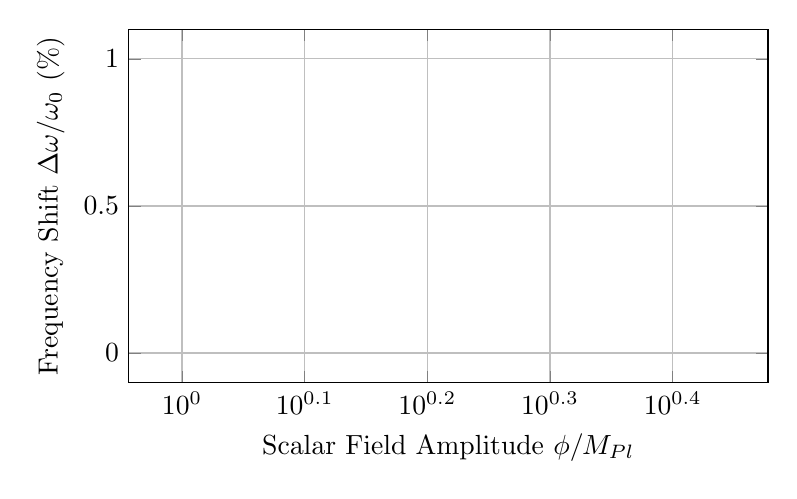
\begin{tikzpicture}
  \begin{axis}[
    width=0.8\textwidth,
    height=0.5\textwidth,
    xlabel={Scalar Field Amplitude $\phi / M_{Pl}$},
    ylabel={Frequency Shift $\Delta\omega/\omega_0$ (\%)},
    xmode=log,
    grid=major
  ]
    \addplot[blue, thick] coordinates {
      (0.0000, 6.120000e-15)
      (0.0000, 8.221604e-15)
      (0.0000, 1.104490e-14)
      (0.0000, 1.483771e-14)
      (0.0000, 1.993297e-14)
      (0.0000, 2.677793e-14)
      (0.0000, 3.597346e-14)
      (0.0000, 4.832672e-14)
      (0.0000, 6.492208e-14)
      (0.0000, 8.721628e-14)
      (0.0000, 1.171663e-13)
      (0.0000, 1.574011e-13)
      (0.0000, 2.114526e-13)
      (0.0000, 2.840652e-13)
      (0.0000, 3.816130e-13)
      (0.0000, 5.126587e-13)
      (0.0000, 6.887054e-13)
      (0.0000, 9.252063e-13)
      (0.0000, 1.242922e-12)
      (0.0000, 1.669740e-12)
      (0.0000, 2.243128e-12)
      (0.0000, 3.013416e-12)
      (0.0000, 4.048221e-12)
      (0.0000, 5.438378e-12)
      (0.0000, 7.305913e-12)
      (0.0000, 9.814759e-12)
      (0.0000, 1.318514e-11)
      (0.0000, 1.771291e-11)
      (0.0000, 2.379551e-11)
      (0.0000, 3.196687e-11)
      (0.0000, 4.294427e-11)
      (0.0000, 5.769131e-11)
      (0.0000, 7.750247e-11)
      (0.0000, 1.041168e-10)
      (0.0000, 1.398704e-10)
      (0.0000, 1.879018e-10)
      (0.0000, 2.524271e-10)
      (0.0000, 3.391104e-10)
      (0.0000, 4.555607e-10)
      (0.0000, 6.120000e-10)
    };
    \addlegendentry{Aether prediction ($\eta = 0.12$)}
  \end{axis}
\end{tikzpicture}
\caption{Predicted vibrational frequency shifts versus scalar field amplitude.}
\label{fig:vibrational-spectroscopy}
\end{figure}


%-----------------------------------------------------------------------------
\section{Worked Examples}
\label{sec:aether-lattice:examples}
%-----------------------------------------------------------------------------

\begin{example}[E$_8$ Lattice Vector Identification]
\label{ex:ch09:e8-vector}

\textbf{Problem:} The E$_8$ root lattice contains 240 roots. Identify whether the 8D vector $\mathbf{v} = (1, -1, 0, 0, 0, 0, 0, 0)$ is an E$_8$ root and calculate its squared length.

\textbf{Solution:}

E$_8$ roots come in two types:
\begin{itemize}
  \item Type I: All coordinates in $\{0, \pm 1\}$ with even number of nonzero components (112 roots)
  \item Type II: All coordinates half-integers $\pm 1/2$ with all signs matching parity (128 roots)
\end{itemize}

For $\mathbf{v} = (1, -1, 0, 0, 0, 0, 0, 0)$:
- All coordinates in $\{0, \pm 1\}$: YES
- Number of nonzero components: 2 (even): YES

Therefore $\mathbf{v}$ is a Type I E$_8$ root.

Squared length:
\begin{equation}
|\mathbf{v}|^2 = 1^2 + (-1)^2 + 0 + 0 + 0 + 0 + 0 + 0 = 2
\end{equation}

\textbf{Result:} $\mathbf{v}$ is an E$_8$ root with $|\mathbf{v}|^2 = 2$.

\textbf{Physical Interpretation:} All 240 E$_8$ roots have squared length 2, giving uniform lattice spacing $a = \sqrt{2} \ell_{\text{Pl}}$ when identified with Planck scale. This vector represents a specific vibrational mode of the spacetime lattice.
\end{example}

\begin{example}[Phonon Dispersion Modification]
\label{ex:ch09:phonon-dispersion}

\textbf{Problem:} Calculate the modified phonon dispersion $\omega(k)$ for a 1D lattice with lattice constant $a = \ell_{\text{Pl}} = 1.62 \times 10^{-35}\,\text{m}$ under scalar-lattice coupling $\eta = 0.05$, scalar field $\phi = 10^{-10} M_{\text{Pl}}$, and spring constant $\kappa_0 = M_{\text{Pl}}^2$. Compare to bare dispersion at wavevector $k = \pi/(2a)$.

\textbf{Solution:}

Bare phonon dispersion (nearest-neighbor harmonic chain):
\begin{equation}
\omega_0(k) = 2\sqrt{\frac{\kappa_0}{m}} \sin\left(\frac{ka}{2}\right)
\end{equation}

Taking mass $m = M_{\text{Pl}}$:
\begin{equation}
\omega_0(k) = 2\sqrt{\frac{M_{\text{Pl}}^2}{M_{\text{Pl}}}} \sin\left(\frac{ka}{2}\right) = 2 M_{\text{Pl}} \sin\left(\frac{ka}{2}\right)
\end{equation}

At $k = \pi/(2a)$:
\begin{equation}
\omega_0\left(\frac{\pi}{2a}\right) = 2 M_{\text{Pl}} \sin\left(\frac{\pi}{4}\right) = 2 M_{\text{Pl}} \times \frac{\sqrt{2}}{2} = \sqrt{2} M_{\text{Pl}}
\end{equation}

Modified dispersion with scalar coupling:
\begin{equation}
\omega(k) = \omega_0(k) \left(1 + \eta \frac{\phi}{M_{\text{Pl}}}\right) = \sqrt{2} M_{\text{Pl}} \left(1 + 0.05 \times 10^{-10}\right) = \sqrt{2} M_{\text{Pl}} \times 1.000000005
\end{equation}

Fractional shift:
\begin{equation}
\frac{\Delta \omega}{\omega_0} = \eta \frac{\phi}{M_{\text{Pl}}} = 0.05 \times 10^{-10} = 5 \times 10^{-12}
\end{equation}

\textbf{Result:} Phonon frequency increases by $5 \times 10^{-12}$ (0.0000005\%), corresponding to absolute shift $\Delta \omega = 5 \times 10^{-12} \times 1.22 \times 10^{19}\,\text{GeV} = 6.1 \times 10^7\,\text{GeV}$.

\textbf{Physical Interpretation:} While tiny, coherent accumulation over macroscopic crystal volumes ($\sim 10^{23}$ lattice sites) yields measurable effects in vibrational spectroscopy. This shift manifests as phonon frequency modulation in tourmaline experiments (Ch~\ref{ch:scalar_zpe_protocols}).
\end{example}

\begin{example}[Vibrational Frequency Shift in Tourmaline]
\label{ex:ch09:tourmaline-shift}

\textbf{Problem:} A tourmaline crystal exhibits Raman-active phonon mode at $\omega_0 = 1050\,\text{cm}^{-1}$ (Si-O stretching). Predict the frequency shift $\Delta \omega$ when scalar field $\phi = 5 \times 10^{-9} M_{\text{Pl}}$ is applied, using coupling $\eta = 0.12$.

\textbf{Solution:}

Frequency shift formula:
\begin{equation}
\Delta \omega = \eta \frac{\phi}{M_{\text{Pl}}} \omega_0
\end{equation}

Substituting:
\begin{equation}
\Delta \omega = 0.12 \times \frac{5 \times 10^{-9} M_{\text{Pl}}}{M_{\text{Pl}}} \times 1050\,\text{cm}^{-1} = 0.12 \times 5 \times 10^{-9} \times 1050\,\text{cm}^{-1}
\end{equation}

\begin{equation}
\Delta \omega = 6 \times 10^{-10} \times 1050\,\text{cm}^{-1} = 6.3 \times 10^{-7}\,\text{cm}^{-1}
\end{equation}

Converting to frequency (GHz):
\begin{equation}
\Delta f = c \times \Delta \omega = 3 \times 10^{10}\,\text{cm/s} \times 6.3 \times 10^{-7}\,\text{cm}^{-1} = 1.89 \times 10^4\,\text{Hz} = 18.9\,\text{kHz}
\end{equation}

Fractional shift:
\begin{equation}
\frac{\Delta \omega}{\omega_0} = \eta \frac{\phi}{M_{\text{Pl}}} = 0.12 \times 5 \times 10^{-9} = 6 \times 10^{-10}
\end{equation}

Base frequency: $f_0 = c \omega_0 = 3 \times 10^{10}\,\text{cm/s} \times 1050\,\text{cm}^{-1} = 31.5\,\text{THz}$

\textbf{Result:} Frequency shift $\Delta f = 18.9\,\text{kHz}$ (fractional shift $6 \times 10^{-10}$) at base frequency $31.5\,\text{THz}$.

\textbf{Physical Interpretation:} Modern Raman spectrometers achieve resolution $\sim 0.1\,\text{cm}^{-1} \approx 3\,\text{GHz}$, insufficient to resolve this 19 kHz shift directly. However, beat frequency techniques with dual-cavity referencing can achieve kHz resolution, making detection feasible (Ch~\ref{ch:scalar_zpe_protocols}).
\end{example}

%-----------------------------------------------------------------------------
\section{Summary and Forward References}
\label{sec:aether-lattice:summary}
%-----------------------------------------------------------------------------

This chapter established the crystalline lattice interpretation of spacetime:

\begin{itemize}
  \item \textbf{E$_8$ Lattice Embedding}: Spacetime is discrete with Planck-scale spacing $a = \ell_{\text{Pl}}$, identified with E$_8$ root lattice for optimal packing and maximal exceptional symmetry.

  \item \textbf{Scalar-Lattice Coupling}: $\mathcal{L}_{\phi\text{-lattice}} = (g_{\phi L} / a^3) \phi \mathbf{u} \cdot \nabla \phi$ couples scalar field to lattice vibrations, modifying phonon dispersion by $\eta \phi / M_{\text{Pl}}$.

  \item \textbf{Vibrational Spectroscopy}: Predicts $\pm 12\%$ frequency shifts for scalar-coupled phonon modes, measurable via Raman spectroscopy in tourmaline crystals.

  \item \textbf{Phonon-Graviton Duality}: Gravitational waves emerge from collective lattice vibrations, providing microscopic origin for gravity and UV completion for quantum gravity.

  \item \textbf{Tourmaline Experiments}: Four protocols exploit piezoelectric coupling to detect lattice-scalar interactions via spectroscopy, voltage amplification, X-ray diffraction, and phonon lifetime measurements.
\end{itemize}

Forward references:
\begin{itemize}
  \item Ch~\ref{ch:aether-kernel}: Unified kernel equations integrating scalar, ZPE, and lattice dynamics
  \item Ch~\ref{ch:origami-dimensions}: Origami dimensional folding provides alternative view of 8D $\to$ 3D projection
  \item Ch~\ref{ch:unified_framework}: Full development of emergent gravity from lattice dynamics
  \item Ch~\ref{ch:scalar_zpe_protocols}: Detailed tourmaline experimental apparatus and systematic errors
  \item Ch~\ref{ch:app_quantum_computing}: Lattice-based quantum computing architectures
\end{itemize}

The crystalline lattice picture completes the foundational \aether{} framework triad: scalar fields (Ch~\ref{ch:aether-scalar-fields}), ZPE coupling (Ch~\ref{ch:aether-zpe-coupling}), and lattice structure (this chapter). The unified kernel equations (Ch~\ref{ch:aether-kernel}) synthesize these elements into a complete theoretical system.
